\documentclass{standalone}
\usepackage{tikz}
\usepackage{tikz-network}
\usepackage{subcaption}
\usepackage{graphicx}
% \usetikzlibrary{graphs, graphdrawing, positioning, quotes}

\begin{document}

% \begin{figure}[H]
% 	\begin{center}
% 		\begin{subfigure}[b]{0.30\textwidth}
		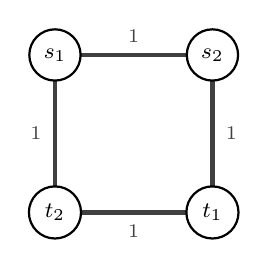
\begin{tikzpicture}
			\coordinate (s1) at (0,0);
			\coordinate (s2) at (2,0);
			\coordinate (t2) at (0,-2);
			\coordinate (t1) at (2,-2);
			\node[draw,circle,fill=white,thick,minimum size=2pt] (CircleNode) at (s1){\footnotesize $s_1$};
			\node[draw,circle,fill=white,thick,minimum size=2pt] (CircleNode) at (s2){\footnotesize $s_2$};
			\node[draw,circle,fill=white,thick,minimum size=2pt] (CircleNode) at (t1){\footnotesize $t_1$};
			\node[draw,circle,fill=white,thick,minimum size=2pt] (CircleNode) at (t2){\footnotesize $t_2$};
			\Edge[label=$1$,position={above=1mm}](s1)(s2)
			\Edge[label=$1$,position={right=1mm}](s2)(t1)
			\Edge[label=$1$,position={below=1mm}](t1)(t2)
			\Edge[label=$1$,position={left=1mm}](t2)(s1)
		\end{tikzpicture}		
		% \caption{Firts subfigure.}
	% 	\label{fig:first}
	% 	\end{subfigure}
	% \begin{subfigure}[b]{0.30\textwidth}
    	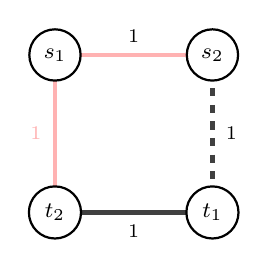
\begin{tikzpicture}
        \coordinate (s1) at (0,0);
        \coordinate (s2) at (2,0);
        \coordinate (t2) at (0,-2);
        \coordinate (t1) at (2,-2);
        \node[draw,circle,fill=white,thick,minimum size=2pt] (CircleNode) at (s1){\footnotesize  $s_1$};
        \node[draw,circle,fill=white,thick,minimum size=2pt] (CircleNode) at (s2){\footnotesize $s_2$};
        \node[draw,circle,fill=white,thick,minimum size=2pt] (CircleNode) at (t1){\footnotesize $t_1$};
        \node[draw,circle,fill=white,thick,minimum size=2pt] (CircleNode) at (t2){\footnotesize $t_2$};
        \Edge[label=$1$,fontcolor=black,color=red!30,position={above=1mm}](s1)(s2)
        \Edge[label=$1$,fontcolor=black,style={dashed},position={right=1mm}](s2)(t1)
        \Edge[label=$1$,fontcolor=black,position={below=1mm}](t1)(t2)
        \Edge[label=$1$,color=red!30,position={left=1mm}](t2)(s1)
    \end{tikzpicture}
	% \caption{Second subfigure.}
	% \label{fig:second}
	% \end{subfigure}
    % \begin{subfigure}[b]{0.30\textwidth}
    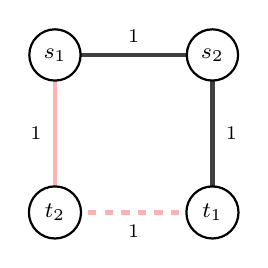
\begin{tikzpicture}
        \coordinate (s1) at (0,0);
        \coordinate (s2) at (2,0);
        \coordinate (t2) at (0,-2);
        \coordinate (t1) at (2,-2);
        \node[draw,circle,fill=white,thick,minimum size=2pt] (CircleNode) at (s1){\footnotesize $s_1$};
        \node[draw,circle,fill=white,thick,minimum size=2pt] (CircleNode) at (s2){\footnotesize $s_2$};
        \node[draw,circle,fill=white,thick,minimum size=2pt] (CircleNode) at (t1){\footnotesize $t_1$};
        \node[draw,circle,fill=white,thick,minimum size=2pt] (CircleNode) at (t2){\footnotesize $t_2$};
        \Edge[label=$1$,fontcolor=black,position={above=1mm}](s1)(s2)
        \Edge[label=$1$,fontcolor=black,position={right=1mm}](s2)(t1)
        \Edge[label=$1$,fontcolor=black,color=red!30, style={dashed},position={below=1mm}](t1)(t2)
        \Edge[label=$1$,fontcolor=black,color=red!30,position={left=1mm}](t2)(s1)
    \end{tikzpicture}   
% 	\caption{Third subfigure.}
% 	\label{fig:third}
% 	\end{subfigure}
% \end{center}
% \caption{A game without pure equilibrium at all}
% \label{fig:noequi}
% \end{figure} 

\end{document}